%=================
\chapter{Sprint 3}
%=================
This chapter explains what the team has done in the third sprint of the 
project. In \autoref{sec:sp3:planning} the planning of this sprint is covered, 
the design is described in \autoref{sec:sp3:design}, together with the user 
stories. The implemented requirements are explained in \autoref{sec:sp3:impl}, 
description of the test done can be found in \autoref{sec:sp3:test}. Through 
the sprint the team has got feedback from the customer, this feedback can be 
found in \autoref{sec:sp3:feedback}.  The results from the evalution of the 
sprint is explained in \autoref{sec:sp3:eval}.

%------------------------
\section{Sprint Planning}
%------------------------
\label{sec:sp3:planning}
For the third sprint we intend to implement the remaining requirements in the product backlog. We feel that the first and second sprint have resulted in a satisfying \gls{utility}, but it is still missing important functionality.

After two sprint iterations, we are still trying to improve our approach to \Gls{scrum}. Each sprint results in new ideas and better ways to do the process, and in this sprint we want everything to be correct and in the right order.\\
\\
There will be two major changes this sprint:
\begin {itemize}
\item We will have a complete planning meeting. The meeting should result in a good planning document, user stories for all the requirements, complete set of work items in the sprint backlog and a early understanding of the design. This approach will be different from earlier sprints, where user stories were written in parallel with implementation. The user story should now be in place before the implementation, and the implementation should be based on the user story. This will make documenting the process easier, and will in turn give the advisors more documentation of what we are doing. Then we can receive valuable feedback from them.

\item In the sprint backlog we will have work items for every task that needs to be done throughout the sprint, including writing minutes, doing documentation, implementation and so on.  Assignment of responsibilities for items in the backlog should not be done at the planning meeting, we rather only give responsibility for one item for each team member at a time. The rest of the items will be unassigned. At each stand-up meeting we pick a task and must be done before the next meeting. This will ensure efficiency and the work done by others are easier to check and revise. It will give us a better work balance, as no team member can gap over too many tasks and leave none for the others.
\end{itemize}
We think that these changes will improve our work efficiency, and make sprint 3 the best one so far.

\subsection{Duration}
%-----------------------
The sprint started with the planning meeting the 19th of October and our work started the following day. The sprint duration is 14 days, and will end the 1st of November with a review meeting. 

\subsection{Sprint Goal}
%-----------------------
For the third sprint the team will update CSjark to version 0.3 which will extend the \gls{utility} so that it contains the complete functionality requested by the customer at this phase of the project. In this sprint we will pick all of the current requirements from the product backlog, as all of the underlying functionality needed for them are already in place from the previous sprints. This means that we will also aim to create a draft of the final design of the system during the sprint.

The most important function that is going to be implemented in this sprint is being able to display \glspl{packet} from different originating platforms properly. This will be implemented by having every \gls{packet} contain a flag specifying their originating platform, and by having our \glspl{dissector} use this flag value to influence how it handles the data in the \gls{packet}.

\subsection{Back Log}
%--------------------
The work items concering features for this sprint are listed in Table \ref{tab:sprint3req}. These are covered by user stories and are about a fourth of the work in this sprint. See the timetable for the other work items.\\
Timetable for this sprint: Table \ref{tab:sprint3time}. \\

\begin{table}[!htb] \small \center
\caption{Sprint 3 Requirement Work Items \label{tab:sprint3req}}
\begin{tabularx}{\textwidth}{l X c c}
	\toprule
	& & \multicolumn{2}{c}{Hours} \\
	\cmidrule(r){3-4}
	User story & Req. and Description & Est. & Act. \\
	\midrule
	\textbf{Impl.} &  & \textbf{56} & \textbf{48} \\
	\hyperref[tab:req:stories7]{US29} & FR5-A: Flags specified for each platform &  5  & 11 \\
	\hyperref[tab:req:stories8]{US31} & FR5-C: \Gls{dissector} support both little and big \gls{endian} & 5  & 4 \\
	\hyperref[tab:req:stories8]{US32} & FR5-D: \Gls{dissector} support different sizes from flags & 12  & 2 \\
	\hyperref[tab:req:stories8]{US33} & FR3-C: Support WIN32, WIN64,\gls{asparc} etc &  5  & 2.5 \\
	\hyperref[tab:req:stories7]{US29} & FR4-B: Configuration supports custom \Gls{lua} files & 6 & 3.5\\
	\hyperref[tab:req:stories7]{US28} & FR2-C: Support \Gls{wireshark} filter and search on attributes &  3 & 1.5\\
	\hyperref[tab:req:stories7]{US29} & FR5-B: \Glspl{dissector} support memory alignment & 4 & 6.5\\
	\hyperref[tab:req:stories7]{US26} & FR1-D: Support \glspl{member} of type \gls{union} & 5  & 6\\
	\hyperref[tab:req:stories7]{US27} & FR2-A add: Display a \gls{wildcard} type for valid \Gls{c} types that \Gls{wireshark} has no support for & 3  & 1.5\\
	\hyperref[tab:req:stories9]{US35} & FR4-D mod: Support specifying the ID of \glspl{dissector} (name and function) & 3  & 3 \\
	\hyperref[tab:req:stories9]{US39} & FR6-D: Don’t regenerate \glspl{dissector} & 1 & 1.5\\
	\hyperref[tab:req:stories7]{US29} & FR2: Handle \Gls{lua} reserved definition names & 2 & 3 \\
	\addlinespace
	\textbf{Testing} &  & \textbf{19} & \textbf{18.5} \\
	 & FR4-B: Custom \Gls{lua} configuration & 2 & 3\\
	 & FR5-C: \Glspl{dissector} support both little and big \gls{endian} & 1 & 1 \\
	 & FR5-D: \Glspl{dissector} support different sizes from flags & 2 & 2 \\
	 & FR3-C: Support WIN32, WIN64, \gls{asparc} etc & 4 & 2.5 \\
	 & FR5-B: \Glspl{dissector} support memory alignement & 8 & 8 \\
	 & FR1-D: Support members of type \gls{union} & 1 & 1 \\
	 & FR2: Handle \Gls{lua} reserved definition names & 1 & 1 \\
	\addlinespace
	\textbf{Doc.} &  & \textbf{11} & \textbf{12} \\
	 & FR4-B: Custom \Gls{lua} configuration & 2 & 3.5\\
	\hyperref[tab:req:stories8]{US34} & FR4-C: Support custom handling of specific data types & 2 & 1.5 \\
	\hyperref[tab:req:stories9]{US36} & FR5: User documentation for what platform that the \gls{utility} support & 3 & 0 \\
	\hyperref[tab:req:stories9]{US37} & FR5: Create developer manual from \Gls{python} docstrings (autodoc plugin) & 4 & 7 \\
	\addlinespace
	\textbf{Fixes} &  & \textbf{16} & \textbf{27} \\
	\midrule
	& Total: & 102 &  105.5\\
	\bottomrule
\end{tabularx}
\end{table}

\begin{table}[!htb] \small \center
\caption{Sprint 3 Timetable\label{tab:sprint3time}}
\begin{tabularx}{\textwidth}{X c c}
	\toprule
	& \multicolumn{2}{c}{Hours} \\
	\cmidrule(r){2-3}
	Description & Est. & Act. \\
	\midrule
	\textbf{Sprint planning} & \textbf{30} & \textbf{47.5} \\
	\addlinespace
	\textbf{Sprint 3 requirements} & \textbf{102} & \textbf{105.5} \\
	Implementation & 56 & 48 \\
	Testing & 19 & 18.5 \\
	User Documentation & 11 & 12 \\
	Fixes & 16 & 27 \\
	\addlinespace
	\textbf{Sprint review} & \textbf{20} & \textbf{18} \\
	\addlinespace
	\textbf{Sprint documentation} & \textbf{75} & \textbf{63} \\
	Sprint 1 document & 10 & 5.5\\
	Sprint 2 document & 14 & 13 \\
	Sprint 3 document & 51 & 44.5 \\
	\addlinespace
	\textbf{Report work} & \textbf{42} & \textbf{52} \\
	User stories to LaTeX & 3 & 4\\
	Architecture update & 8 & 6.5\\
	Glossaries and acronyms & 16 & 20\\
	Requirement review & 15 & -\\
	Layout and correction & 15 & 6.5 \\
	\addlinespace
	\textbf{Lectures} & \textbf{21} & \textbf{14} \\
	\addlinespace
	\textbf{Presentation outline} & \textbf{2} & \textbf{2} \\
	\addlinespace
	\textbf{Meetings} & \textbf{57} & \textbf{45} \\
	Advisor meetings & 28 & 21 \\
	Customer meetings & 8 & 5 \\
	Stand-up meetings & 21 & 19 \\
	\textbf{Project management} & \textbf{20} & \textbf{14} \\
	\midrule
	Total: & 367 & 361 \\
	\bottomrule
\end{tabularx}
\end{table}

%----------------------
\section{System Design}
%----------------------
\label{sec:sp3:design}
The system design defines the new modules and architecture that has to be in place to satisfy the specified requirements that we have included in the sprint 3 backlog. Most of the design are already done in earlier sprints; now we extend that and add some new elements.

\subsection{System overview}
%----------------------
Now that the \gls{utility} has both basic and advanced features, it is time to specialize and make support for environmental variables that can be found in Thales' source code. This basically include various platform specific support, \gls{endian} handling and minor technicalities. The latter one is vital for the customer in order for the \gls{utility} to be efficient and adequate. \\
\\
The new design resulted in both major and minor changes to the class diagram, see \autoref{fig:ClassDiagramSprint3}.
\begin{figure}[!htb]
	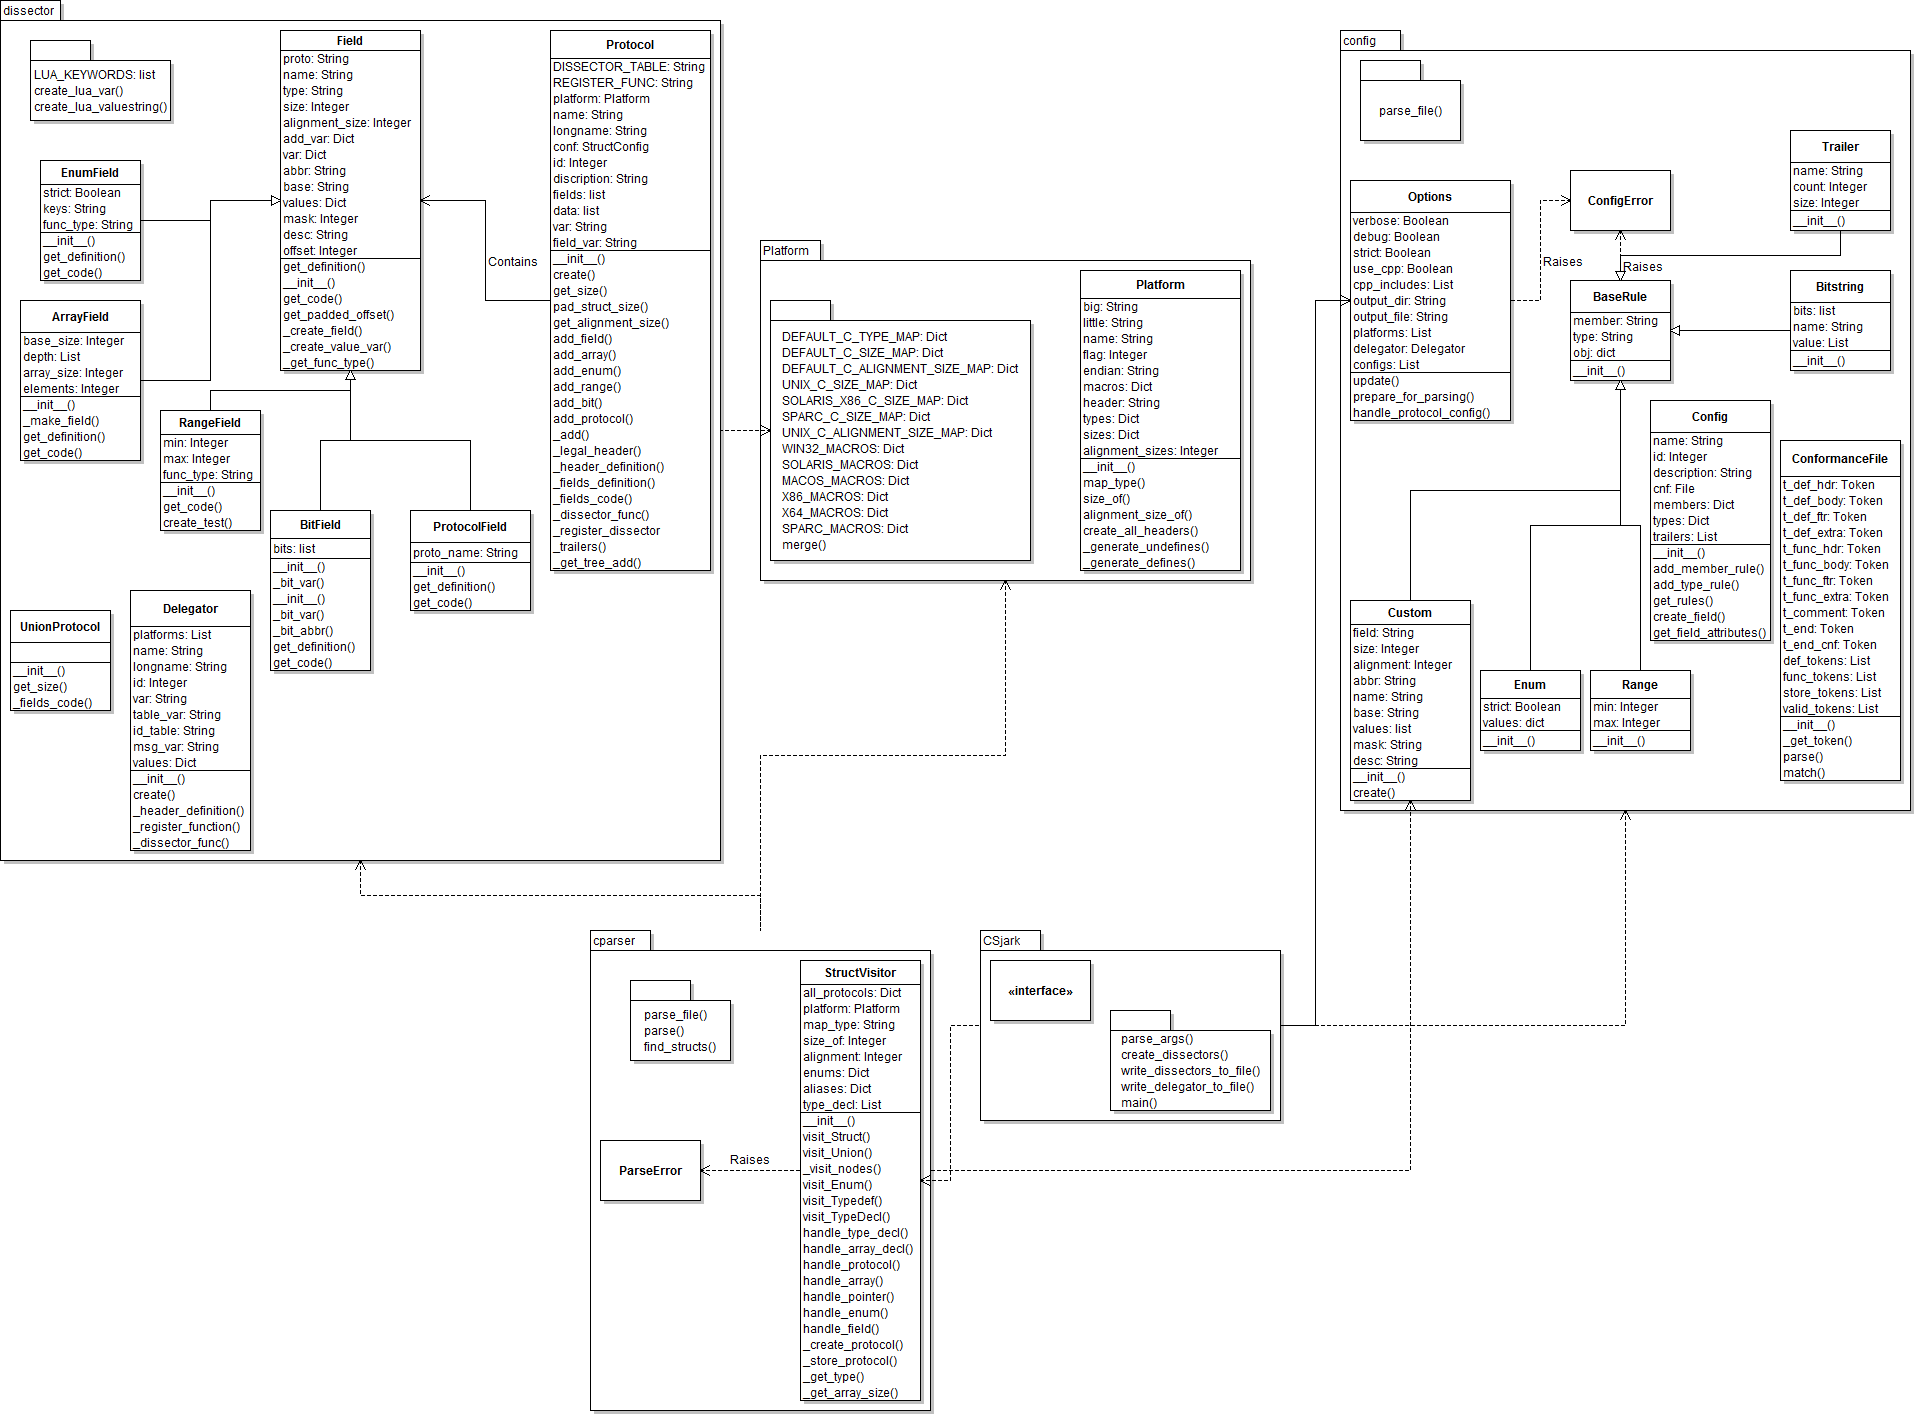
\includegraphics[width=\textwidth]{./sprints/img/class_diagram_s3}
	\caption{Sprint 3 class diagram\label{fig:ClassDiagramSprint3}}
\end{figure}

\paragraph{Major changes}
\begin{itemize}
\item New module called Platform, to hold platform specific information. Ealier some information about the platform were stored in the config module, but now we have so extensive platform specifications that it is best to separate it in its own module. See the section regarding platform specific support for more info.
\item Moved the \gls{cli} class from csjark to config, and renamed it to Options. This class holds the attributes passed from the command line interface. This will make the code more loosely coupled now that the configuration attributes are stored in the correct module. 
\item A delegator class was added to \gls{dissector} module. This class will be responsible for delegating dissecting to \glspl{protocol}. It will be a top-level \gls{dissector} that delegates the task of dissecting specific messages to \glspl{dissector} generated by \gls{protocol} instances. It will be responisble for finding the correct \gls{dissector} for a message based on the origin of it.
\item UnionProtocol class was added to the \gls{dissector} module. This class willl be responsible for holding the \gls{union} and its \glspl{member}. Now the \gls{utility} will be able to handle \glspl{union}. 
\item In the config module the class StructConfig was removed and replaced by Options and Config. As mentioned, Options holds the attributes submitted from the commandline or attributes loaded by one or more config-files. Config holds the configuration for a specific \gls{protocol}.

\end{itemize}

\paragraph{Minor changes}
\begin{itemize}
\item Config now only have one method.
\item In the ConformanceFile, tokens and methods have been added.
\item Trailers have a name variable.
\item In the ProtocolField in the \gls{dissector} module, the \gls{protocol} is stored with a name instead of id. This has been pointed out by Thales as the correct way to do it.
\item Methods have been added to different classes to support the major changes. This is a change, more than an addition of new elements. 
\end{itemize}

\subsubsection{Platform specific support}
We know that the various platforms behave differently, and this must be supported by our \gls{utility}. The customer has mentioned at least three platforms that we have to support. As we emphasize extensibility and modifiability, it must also be expected that new platforms will be added or removed to the supported platforms in the future. Thereby we will try to make the set-up for support easily understandable.

We have decided that the platform definition will be a subpart of a flag-field in the \glspl{struct} \gls{header}. To ensure modifiability we will assign a 16 bit field for this, giving the developers possibility to have 65536 unique platforms. We will make the platform flag point to the platform module which has the following information about the actual platform:
\begin{itemize}
\item \Gls{endianness}
\item Length of fields
\item Memory alignment
\item Macros
\item Types
\end{itemize}
All of these fields must be combined to enable the \gls{utility} to generate a \gls{dissector} that will dissect the \gls{struct} correctly.

\subsubsection{Dictionary lookup}
Deciding how to implement handling of different platforms ended in a design draft seen in \autoref{fig:platformhandling}. The \gls{dissector} module will make a dictionary lookup in the table of supported platforms. This table conatins all platforms that the \gls{utility} can make \glspl{dissector} for, and their information of how the \gls{dissector} shall be encoded to achieve correct handling of \gls{endianness}, length of fields and memory alignment.
We will start out by hardcoding this into the source code, but in the end we want to have this feed to the \gls{utility} through a configuration-file which will be stored in the platform module. This is the way the customer has envisioned it.  

\begin{figure}[!htb]
	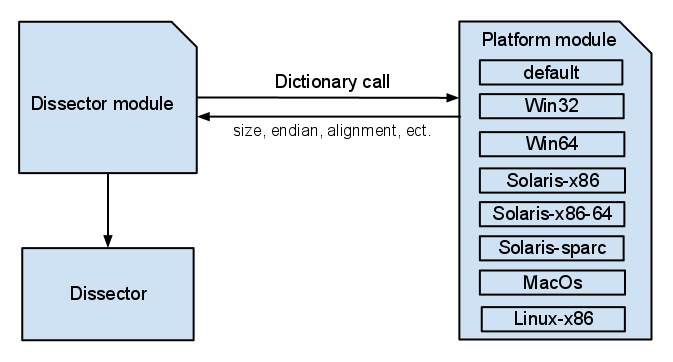
\includegraphics[width=\textwidth]{./sprints/img/platformhandling}
	\caption{Platform handling\label{fig:platformhandling}}
\end{figure}

\subsubsection{\Gls{endianness}}
An important feature is the support for different \gls{endian} handling. \Gls{endianness} defines how the bytes are ordered. Big and little endian tells which bit that is the most significant, and thereby the value that the bits represent. \autoref{fig:endianness} show the differnce between big and little endian.
\begin{figure}[!htb]
	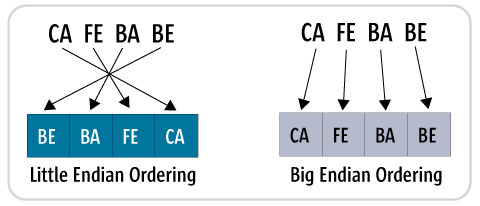
\includegraphics[width=\textwidth]{./sprints/img/endianness}
	\caption{\Gls{endianness}\cite{Endianness} \label{fig:endianness}}
\end{figure}
\Gls{wireshark} has built-in support for reading big and little \gls{endian}, and the dissector will tell which it should use. When the \gls{dissector} module builds the abstract syntacs tree, it must call the platform module to see what \gls{endian} it shall use. In the class diagram the \gls{dissector} module imports the platform module, from there it gets the information it needs regarding the \gls{endianness}. 

\subsubsection{Filter and search in \Gls{wireshark}}
The amount of data that are collected and dissected can be very large. The need for a filter and search mechanism is apparent. \Gls{wireshark} has this built-in, and the customer want the \gls{utility} to support it. The abbrevations will be set for each field and generated by the \gls{dissector} module. \Gls{wireshark} collects these when the actual \gls{dissector} is used, and then a user will be able to search for them. In the design we have emphesized and assured us that the chosen abbrevations are descriptive, as the customer has stated it important in earlier customer meetings. 

\subsubsection{\Gls{batch processing}}
The \gls{batch processing} was implemented in the second sprint, but we have to modified it to ensure efficiency and reliability. When the \gls{utility} encounter a \gls{header} that it can not parse, it should skip that and move on to the next \gls{header} in the queue. This will make the \gls{utility} able to process almost all the \glspl{header} in one bacth, and ensure reliability. This is also according to the customers specification.

The redesign of the config module will ensure better efficiency when the batch process is executed. It will also be easier to trace the connection between configuration and options. 

\subsection{User stories}
\label{sec:req:stories3}
This section lists the user stories for the third sprint, these are displayed in \autoref{tab:req:stories7}, \autoref{tab:req:stories8} and \autoref{tab:req:stories9}.
As we are developing a very technical \gls{utility} we have written user stories with an implementation level of abstraction. 
These user stories represent how we intend to add the functionality of each requirement to the \gls{utility}.
The administrator in this context is the administrator at Thales Norway AS. 
The developer is the person that uses \Gls{wireshark} with the \gls{dissector} generated by CSjark.

\begin{table}[htbp] \footnotesize \center
\caption{User stories - Sprint 3 part 1\label{tab:req:stories7}}
\noindent\makebox[\textwidth]{%
\begin{tabularx}{1.2\textwidth}{l X}
	\toprule
	Header & Value \\
	\midrule
	ID & US26 \\
	Requirement & FR1-D: The \gls{utility} must support \glspl{member} of type \gls{union} \\
	What & The administrator wants to generate \glspl{dissector} which contain \glspl{struct} with \glspl{union} as \glspl{member}. \\
	How & When the administrator feeds the \gls{utility} with a \gls{header} containing a \gls{union}, the cparser module should parse the \gls{union} and its \glspl{member} to find the total size of the 
	\gls{union} (which equals the size of the largest \gls{member}), and then create an instance of UnionField from the \gls{dissector} module representing the \gls{union} and its \gls{member}\\
	Result & The \gls{utility} support \gls{union} \glspl{member} in \glspl{struct}. \\
	\midrule
	ID & US27 \\
	Requirement & FR2-A\textit{Addition:} Display a \gls{wildcard} type for valid \Gls{c} types that \Gls{wireshark} has no support for. \\
	What & The administrator should be able to give the tool a \gls{struct} with a valid \Gls{c}-type even if \Gls{wireshark} does not have a way to display that type in a natural way.
	The \gls{dissector} should the just display the name of the type, the name of the \gls{member} and the hex value from the \gls{packet}. \\
	How & The \gls{parser} module will recognise if a type it encounters are supported in \Gls{wireshark} or not. If it is not supported, it will add a \gls{wildcard} field to the prototype object
	representing the enclosing \gls{struct}. \\
	Result & The administrator will be able to both run the \gls{utility} and get some information from the \gls{dissector} even if the type used is not supported by \Gls{wireshark}. \\
	\midrule
	ID & US28 \\
	Requirement & FR2-C: Filter and search on attributes (important to have descriptive abbreviations) \\
	What & The developer wants to find specific attributes in \Gls{wireshark}. The amount of data captured can be big.
	After the \glspl{packet} have been dissected, they are presented in \Gls{wireshark}. The developer will have a hard time finding 
	attributes by manual seeking. The built-in search and filter functionality needs to be supported to accommodate the developer. \\
	How & The functionality is already in \Gls{wireshark}. To utilize it, an abbreviation field must be provided to \Gls{wireshark}. This abbreviation field will be in the \gls{dissector} module
	and is included in the \gls{dissector} generated by the \gls{utility}. When \Gls{wireshark} runs the \gls{dissector}, all abbreviations are collected which will make it possible to filter and search
	on attributes. \\
	Result & The developer will be able to search and filter by attributes. \\
	\midrule
	ID & US29 \\
	Requirement & FR5-A: Flags must be specified in configuration for each platform \\
	What & The administrator wants to generate \glspl{dissector} which are different depending on platform. \\
	How & To be able to create \glspl{dissector} which are different depending on the originating platform, the administrator needs to specify in the configuration which platforms he wants to support.
	The config module should accept such configuration and store it so other modules can use it. \\ 
	Result & The administrator can specify what platform he is using by setting a flag in the configuration. \\
	\midrule
\end{tabularx}}
\end{table}

\begin{table}[htbp] \footnotesize \center
\caption{User stories - Sprint 3 part 2\label{tab:req:stories8}}
\noindent\makebox[\textwidth]{%
\begin{tabularx}{1.2\textwidth}{l X}
	\toprule
	Header & Value \\
	\midrule
	ID & US31 \\
	Requirement & FR5-C: Generate \glspl{dissector} which support both little and big \gls{endian} platforms \\
	What & The administrator wants \glspl{dissector} which handle both big and little \gls{endian} encoding. \\
	How & The \gls{dissector} module will need to create different \Gls{lua} code for big and little \gls{endian}, when adding nodes to the \Gls{wireshark} tree and when calling other \glspl{dissector}.
	The \gls{dissector} module shall have functionality which generates \Gls{lua} code depending on \gls{endianness}, and the different Field classes must use this function when adding 
	nodes to the \Gls{wireshark} tree. \\
	Result & \Glspl{dissector} can be created with platform specific \gls{endian}. \\
	\midrule
	ID & US32 \\
	Requirement & FR5-D: Generate \glspl{dissector} which support different sizes depending on platforms \\
	What & The administrator wants to generate \glspl{dissector} for \gls{struct} where \glspl{member} size depend on the originating platform. \\
	How & When the administrator feeds the \gls{utility} a \gls{header} file and a config file with a set of platform he wants \glspl{dissector} for, the config module will create new \gls{header} files
	with \Gls{c} \gls{preprocessor} directives for each platform. These files should define platform-specific macros which emulates parsing on the specific platform. 
	The \gls{dissector} module then create different \glspl{dissector} for each message on each platform, and a mapping is added inside the master \Gls{lua} file which maps message id and
	platform to the correct \gls{dissector}. \\
	Result & \Glspl{dissector} can be created with platform specific sizes of \glspl{member}.\\
	\midrule
	ID & US33 \\
	Requirement & FR3-C: Support for configuring a platform with a platform specific macro like WIN32, \_WIN64, \_\_sparc to be able to  support different \gls{struct} definitions 
	for different platforms. \\
	What & The administratorwants to be able to configure the \gls{utility} to make \glspl{dissector} that support \glspl{struct} that is defined differently on different platforms via platform specific
	macros like WIN32, \_WIN64, \_\_sparc. \\
	How & The administrator specify the macro associated with a platform together with the platform definition configuration. The \gls{utility} then make an auxiliary \gls{header} file for each 
	platform configuration with the specified macro definition. These \glspl{header} are forwarded to the \gls{parser} module, which uses them to generate
  	one \gls{dissector} for each platform for each \gls{struct}. All \glspl{dissector} dissecting the same \glspl{struct} are stored in the same file, but are added to a platform specific \gls{dissector} table. \\
	Result & The generated \Gls{lua} files corresponding to \glspl{struct} now includes one \gls{dissector} for each platform defined in the configuration file. \\
	\midrule
	ID & US34 \\
	User doc & FR4-C: User documentation for configurating custom handling of specific types. \\
	What & The administrator should be able to find out how to specify custom handling for a specific type by reading the user documentation. \\
	How &	 The administrator opens the user documentation and finds the section about configuration. From here he locates the sub section about custom type handling. 
	This section gives a good description of how to write such configuration and what kind of configuration that could be done. There should also be some examples to clarify
	the description. After reading the section, the user has a good idea of how to do the desired custom handling. \\ 
	Result & The administrator is able to use custom handling of specific types. \\
	\midrule

\end{tabularx}}
\end{table}

\begin{table}[htbp] \footnotesize \center
\caption{User stories - Sprint 3 part 3\label{tab:req:stories9}}
\noindent\makebox[\textwidth]{%
\begin{tabularx}{1.2\textwidth}{l X}
	\toprule
	Header & Value \\
	\midrule
	ID & US35 \\
	Requirement & FR4-D modified: Configuration must support specifying the ID of \glspl{dissector} \\
	What & The administrator wants to specify the ID of a \gls{dissector} in a configuration file. The \glspl{dissector} should not be given any ID if it has not been specifically configured. \\
	How & When the cparser finds a \gls{struct} in the \gls{AST} it looks for a configuration file for the \gls{struct}. If a config-file is found, the	ID of the prototype field
	representing the \gls{dissector} will be mapped to the ID given in the config-file.  If it is not found, the ID will be sat to NONE. \\
	Result & The administrator can specify the ID of \glspl{dissector} in the configuration. \\
	\midrule
	ID & US36 \\
	User doc & FR5 User documentation for how to add or remove support for a platform in the \glspl{dissector} generated from the \glspl{utility}. \\
	What & The administrator should be able to find out how to add or remove support for a platform in the \glspl{dissector} by reading the user documentation. \\
	How & The administrator opens the user documentation and finds the section about configuration. From here he locates the sub section about platform support. 
	This section gives a good description of how to add or remove support for a platform in the configuration, so that the administrator understands how to do
	this after reading the section. \\
	Result & The administrator is now able to configure the \gls{utility} to add or remove platform support from the generated \glspl{dissector}. \\
	\midrule
	ID & US37 \\
	User doc & FR5 User documentation for what platform that the \gls{utility} support. \\
	What & The administrator should be able to find out what platforms he can add support for in the custom \gls{dissector} files. \\
	How & The administrator opens the user documentation and finds the section about configuration. From here he locates the sub section about platform support.
	This section gives a list of currently supported platforms by the \gls{utility}. It should also have some information of where to	find the documentation that describes
	how to add support for more platforms. \\
	Result & The administrator is now able to look up what platforms he can get the \glspl{dissector} to support. \\
	\midrule
	ID & US38 \\
	Requirement & FR6-D The \gls{utility} should not regenerate \glspl{dissector} within a single run. \\
	What & The administrator should be able to specify folder that includes both a standalone \gls{header} file with a \gls{struct} definitions and another \gls{header} file that includes
	the first \gls{header}. The \gls{utility} will only generate the \gls{dissector} once for the \gls{struct} inside the first \gls{header}. \\
	How & For each \gls{struct} encountered, the \gls{utility} will check the table of generated \glspl{dissector} to see if there is an existing \gls{dissector} generated for the \gls{struct} name.
	It will only generate a new \gls{dissector} if the table of \glspl{dissector} is empty for that name. \\
	Result & The \gls{utility} will run faster as a result of not needing to regenerate \glspl{dissector}. \\
	\midrule
	ID & US39 \\
	Requirement & Handle \Gls{lua} reserved definition names \\
	What & The \Gls{c} \glspl{struct} could contain \glspl{member} with names that are reserved by \Gls{lua}. The \gls{dissector} module needs to avoid creating \Gls{lua} variables with such names.  \\
	How &	 The \gls{dissector} module has a method called create\_lua\_var. This method will ensure that variable names are valid, by comparing the variable names to a list
	of \Gls{lua} reserved keywords, and if there is a match we need to add an underscore in front of the variable name. \\ 
	Result & The \gls{utility} can handle \Gls{c} \gls{header} files that contain \Gls{lua} reserved definition names. \\
	\bottomrule
\end{tabularx}}
\end{table}

\begin{table}[htbp] \footnotesize \center
\caption{User stories - Sprint 3 part 4\label{tab:req:stories10}}
\noindent\makebox[\textwidth]{%
\begin{tabularx}{1.2\textwidth}{l X}
	\toprule
	Header & Value \\
	\midrule
	ID & US40 \\
	Requirement &  FR5-B: Generate \glspl{dissector} with correct alignment depending on platform \\
	What & The administrator wants to generate \glspl{dissector} which are different depending on platform. \\
	How & The \gls{dissector} module will use the configured flags from the config module to modify the generated \Gls{lua} \glspl{dissector} so that they have the right memory structure alignment and \gls{endianness}.
	The \gls{dissector} module shall have a function which calculates the offset for each field to align it, and functions which creates fields for specific \gls{endianness}. \\
	Result & \Glspl{dissector} can be created with platform specific memory structure alignment \\
	\bottomrule
\end{tabularx}}
\end{table}


%-----------------------
\section{Implementation}
%-----------------------
\label{sec:sp3:impl}
The main focus in this sprint was to add support for different platforms. Several 
things are dependent on platform; \gls{endianness}, the memory allingment and sizes 
of data types. It is also possible that \glspl{struct} can be defined differently for 
each platform. The \gls{utility} will generate different \glspl{dissector} for each 
platform. A \gls{dissector} will detect the platform and use the correct 
platform \gls{dissector}.

Support for the \gls{union} data type, finishing implementation of custom \Gls{lua} files 
and modification of functionallity implemented in the previous sprint was also 
done in this sprint.

\subsection{Specify Flags for Each Platform}
%-----------------------
It is necessary to specify flags for each platform to make it possible to 
correctly detect and display packages that wireshark captures. In wireshark 
the flags are used to tell which platform the \gls{packet} is sent from, so that 
the right \gls{dissector} is used to display the \glspl{packet} in \Gls{wireshark}. In the 
\gls{utility} the flag points to what kind of \gls{endianness}, how memory is aligned and 
the different sizes that is used for data types on the platform. These data 
are used to genereate a \gls{dissector} for the specific platform. The 
luastructs protocol will read the platform flag, an find the dissector for the 
platform.

\subsection{Support Little and Big \Gls{endian}}
%-----------------------
Different platforms can order bytes in either little(left-to-right) or 
big(right-to-left) \gls{endian}. The \Gls{Windows} platform uses little \gls{endian}, and \gls{asparc} 
uses big \gls{endian}. Since the \gls{utility} has to support both platforms, it was 
necessary to support handling of \gls{endianness}. The \Gls{lua} \gls{api} in \Gls{wireshark} has 
functionallity to display data in both little and big \gls{endian}. Therefore the 
\gls{utility} has to read the specfied flag for the platform, and generate a \Gls{lua} 
\gls{dissector} that displays the data correctly for the given platform.

\subsection{Support Different Sizes from Flags}
%-----------------------
On different platforms, there can be different sizes on the data types. For 
example on windows a \emph{long double} is 8 bytes, and on \gls{asparc} it is 16 
bytes. It is possible to specify sizes for data types for each platform. All 
these specifications is written in \Gls{python} code, and are easy to modify for the 
user of the system.

\subsection{Support Platform Specific Macros}
%-----------------------
All \Gls{c} compilers have predefined macros for different operating systems and 
processors. These macros are much used in code that need to be portabel for 
different platforms. When using these macros it is possible to create 
different \gls{struct} \glspl{member} for each operating system, as shown in 
\autoref{code:predefmacro}, which will use different data types on each 
operating system. All platform specific macros are specified for each 
platform, so the \gls{dissector} is generated correctly for each of the platforms. 
Currently all the platform specifications is done in \Gls{python} code.

\lstset{language=C,caption={Macros in C},label=code:predefmacro}
\lstinputlisting[language=C]{./sprints/code/predefmacro.h}

\subsection{Support Custom \Gls{lua} Files}
%-----------------------
Implementation of this feature started in sprint 2, and support for using 
conformance file to add \Gls{lua} code to correct places in the \Gls{lua} \gls{dissector} was 
finished in this sprint. With the conformance file it is possible to add code 
before and after an \gls{member} in both the definition and function part of the 
\gls{dissector}. It also possible to replace the code for a \gls{member} in both of these 
sections. In the example below there is written custom \Gls{lua} for a 
\gls{struct}(temperature) with on \gls{integer} \gls{member} (celsius). In the conformance file 
in \autoref{code:customcnf} there added three lines of comments as a custom 
\Gls{lua} code, that are going to be added to the \Gls{lua} \gls{dissector}. In 
\autoref{code:customlua} it is possible to see the custom \Gls{lua} code that was 
added to the \Gls{lua} \gls{dissector}. The first comment is added after the \gls{member} 
definition. The two other comments are added above and below the \gls{member} in the 
function part of the \Gls{lua} \gls{dissector}.

\lstset{language=C,caption={Custom Lua conformance file},label=code:customcnf}
\lstinputlisting[language=C]{./sprints/code/custom.cnf}

\lstset{language=C,caption={Custom Lua dissector code},label=code:customlua}
\lstinputlisting[language=C]{./sprints/code/custom.lua}

\subsection{Support \Gls{wireshark} Filter and Search}
%-----------------------
\Gls{wireshark} has a display filter, where it is possible to use \gls{packet} filtering. 
Each field in our generated \glspl{dissector} has a abbrevation name that is 
connected to a \gls{struct}. For each \gls{member} of a \gls{struct}, it is possible to filter 
on a value. An example is shown in \autoref{fig:wsfilter}, this shows a 
filtering for \glspl{packet} where Trondheim is equal to the \gls{member} \emph{place} in 
the \gls{struct} \emph{postcode}. 

\begin{figure}[ht]
	\center
	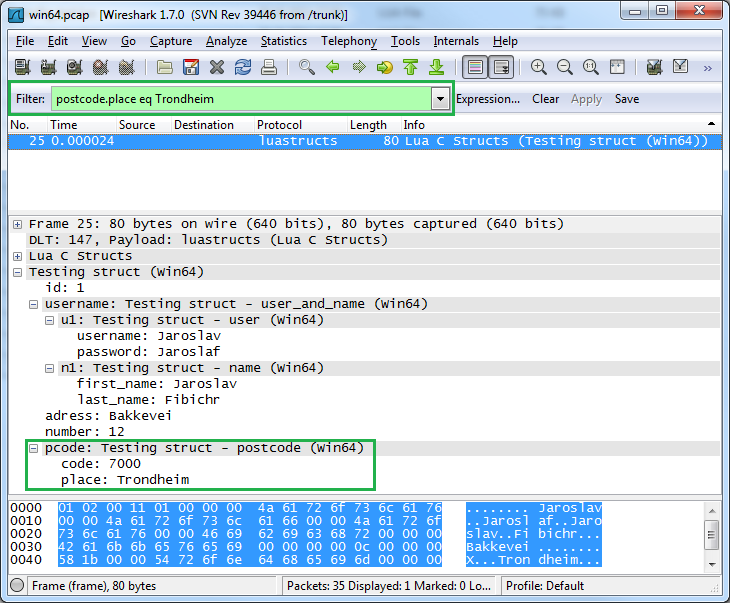
\includegraphics[width=\textwidth]{./sprints/img/wireshark_filter}
	\caption{Union type support\label{fig:wsfilter}}
\end{figure}

\subsection{Support Different Memory Alignment}
%-----------------------
Since the \glspl{dissector} generated by the \gls{utility}, are going to be used for 
inter-process commuincation, it is important to handle memory structure 
alignment, because the \gls{packet} that \Gls{wireshark} capture is only a copy of the 
memory. Memory alignment is how the data are stored in the memory. Each \gls{member} 
of a structure has a alignment. With the correct handling of memory alignment it is 
possible to display the \glspl{struct} correctly in \Gls{wireshark}.

\subsection{Support Union Type}
%-----------------------
The \gls{union} type is a \gls{member} that can contain different data types with 
different sizes. The \gls{union} will allocate memory for the largest type defined 
in the \gls{union}. \autoref{code:union} shows an example of a \gls{header}-file with a 
\gls{union} type. The compiler is responsible for keeping track of size and 
alignment requirements\cite[p.147]{Kerninghan1988} . Since it is not 
possible to find out which data type that is used in \Gls{wireshark}, the \gls{utility} 
has to generate a \gls{dissector} that displays the values for each data type. 
\autoref{fig:wsunion} displays the \gls{dissector} generated from the \gls{struct} in 
\autoref{code:union}. This shows the \gls{union} with three \glspl{member}, all of them are 
listed with their values. In this case the \gls{float} value is the correct one.

\begin{figure}[ht]
	\center
	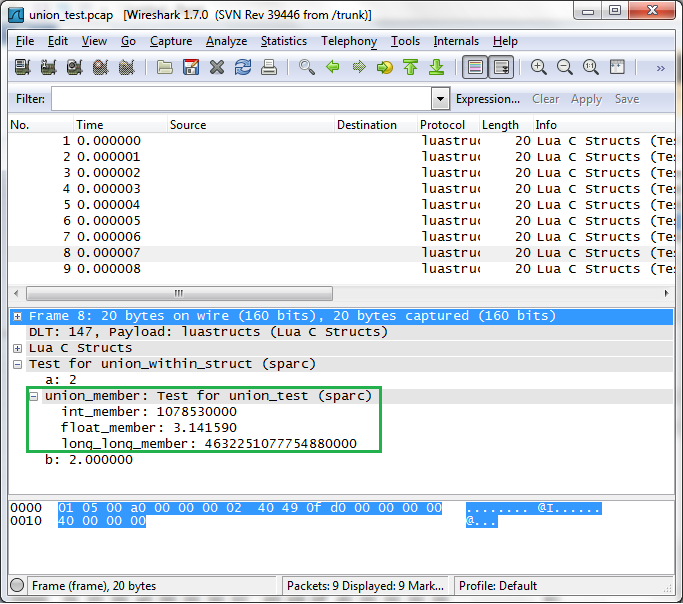
\includegraphics[width=\textwidth]{./sprints/img/wireshark_union}
	\caption{Union type support\label{fig:wsunion}}
\end{figure}

\lstset{language=C,caption={Union type},label=code:union}
\lstinputlisting[language=C]{./sprints/code/union.h}

\subsection{Display Types \Gls{wireshark} Do Not Support}
%-----------------------
The \gls{utility} is able to genereate \glspl{dissector} for \Gls{c} data types, that \Gls{wireshark} 
do not support. When such a data type occur, \Gls{wireshark} will display only 
display the \gls{packet} data. An example of a data type, which \Gls{wireshark} do not 
support is \emph{long double} on the \gls{asparc} platform, which is a 128-bit foat. 
For this \Gls{wireshark} will display the 16 bytes in \gls{hexadecimal}.

\subsection{Support Specifying ID of \Glspl{dissector}}
%-----------------------
Specifying \gls{dissector} ID has been modified from sprint 2. The \gls{dissector} will 
still use the ID given in the configuration for a \gls{struct}, if the \gls{struct} is not 
given an ID in the configuration, then the ID for the \gls{struct} will be set to 
\emph{NONE}. This is done to ensure that \glspl{struct} have an unique ID for their 
\gls{dissector}. \Glspl{struct}-in-\glspl{struct} \gls{member} do not need an ID since they are called 
from the \gls{struct}' by the \gls{dissector} name.

\subsection{Do Not Regenerate \glspl{dissector}}
%-----------------------
To increase the performance on generation of \glspl{dissector}, \glspl{dissector} that 
allready are genereated in \gls{batch mode}, will only be generated once in a batch 
mode execution. This feature will be improved in the next sprint, so it only 
genereates \glspl{dissector} in \gls{batch mode} that are modified or new since the last 
batch run.

\subsection{Handle \Gls{lua} Reserved Keywords}
%-----------------------
\Gls{lua} has a list of reserved keywords, and some of these keywords are allowed in 
the \Gls{c} language. The \gls{utility} is able to support this under generation of \Gls{lua} 
code, when an identifier is a lua keyword, an underscore(\_) is added, so the 
identifier start with ''\_''.

\subsection{Support for Complex \Glspl{array}}
%-----------------------
Support for typedef was implemented in the previous sprint, in this sprint it 
has been improved to also support type definitions of complex \glspl{array}. Support 
for type definition of array is implemented, an example of such type 
definition in \Gls{c} is shown in \autoref{code:typedefarray}. Also support for 
\glspl{array} of \glspl{enum}, \glspl{array}, \glspl{struct} and pointers has been added.

\lstset{language=C,caption={Typedef of arrays},label=code:typedefarray}
\lstinputlisting[language=C]{./sprints/code/typedefarray.h}


%-----------------------
\section{Sprint Testing}
%-----------------------
\label{sec:sp3:test}
During sprint 3 the team executed a total of 11 test cases, but no additional testing features were added during the sprint. The test cases executed in this sprint can be found in \autoref{sec:testcases}. An example of such a test case can be seen in \autoref{tab:STID15} while the rest of the test cases can be found in the listing below:

\begin{itemize}
	\item TID15 - Supporting \gls{batch mode} of \Gls{c} \gls{header} and configuration files \autoref{tab:sp3TID15}
	\item TID16 - Supporting custom \Gls{lua} configuration \autoref{tab:sp3TID16}
	\item TID17 - Supporting \glspl{union} \autoref{tab:sp3TID17}
	\item TID18 - Supporting filter and search in \Gls{wireshark} \autoref{tab:sp3TID18}
	\item TID19 - Supporting WIN32, \_WIN64, \_\gls{asparc} etc \autoref{tab:sp3TID19}
	\item TID20 -  Supporting the use of flags specifying platforms to display \gls{member} values correctly \autoref{tab:sp3TID20}
	\item TID21 - Supporting platforms with different \glspl{endian} \autoref{tab:sp3TID21}
	\item TID22 - Supporting alignments \autoref{tab:sp3TID22}
	\item TID 23 - Handling \Gls{lua} keywords \autoref{tab:sp3TID23}
	\item TID24 - Sprint 3 functionality test \autoref{tab:sp3TID24}
	\item TID25 - Sprint 3 requirements test \autoref{tab:sp3TID25}
\end{itemize}

\begin{table}[ht] \footnotesize \center
\caption{Test case TID15}\label{tab:STID15}
\noindent\makebox[\textwidth]{%
\begin{tabularx}{1.2\textwidth}{l X}
	\toprule
	Header & Description \\
	\midrule
	Description & Support \gls{batch mode} of \Gls{c} \gls{header} and configuration files \\
	Tester & Lars Solvoll Tønder \\
	Prerequisites & The \gls{utility} has have been installed on the system, there also needs to exist a header and configuration file for this test \\
	Feature &  Test that the \gls{utility} is able to genereate \glspl{dissector} for all \gls{header}-files in a folder, with configuration\\
	\midrule
	\multirow{2}{*}{Execution} & 1. Feed the \gls{utility} the name of the two folders with \gls{header}-files and configuration-files. \\
	& 2. Read output from the \gls{utility} \\
	\midrule
	Expected result  & 2. The \gls{utility} should provide the user with the amount of \gls{header} files processed and the number of \glspl{dissector} created. It should also provide the user with error messages for the \gls{header} and configuration files it was unable to run  \\
	\bottomrule
\end{tabularx}}
\end{table}

\subsection{Test Results}

\begin{table}[!htb] \footnotesize \center
\caption{Supporting \gls{batch mode} of \Gls{c}-\glspl{header} and configuration files\label{tab:sp3TID15}}
\begin{tabular}{l l}
	\toprule
	Header & Description \\
	\midrule
	Description & Supporting \gls{batch mode} of \Gls{c} \gls{header} and configuration files \\
	Tester & Lars Solvoll Tønder \\
	Date & 28.10.2011 \\
	Result & Success\\
	\bottomrule
\end{tabular}
\end{table}

\begin{table}[!htb] \footnotesize \center
\caption{Supporting custom \Gls{lua} configuration\label{tab:sp3TID16}}
\begin{tabular}{l l}
	\toprule
	Header & Description \\
	\midrule
	Description & Supporting custom \Gls{lua} configuration\\
	Tester & Lars Solvoll Tønder \\
	Date & 30.10.2011\\
	Result & success\\
	\bottomrule
\end{tabular}
\end{table}

\begin{table}[!htb] \footnotesize \center
\caption{Supporting \glspl{union}\label{tab:sp3TID17}}
\begin{tabular}{l l}
	\toprule
	Header & Description \\
	\midrule
	Description & Supporting \glspl{union}\\
	Tester & Lars Solvoll Tønder\\
	Date & 30.10.2011\\
	Result & success\\
	\bottomrule
\end{tabular}
\end{table}

\begin{table}[!htb] \footnotesize \center
\caption{Supporting filter and search in \Gls{wireshark}\label{tab:sp3TID18}}
\begin{tabular}{l l}
	\toprule
	Header & Description \\
	\midrule
	Description & Supporting filter and search in \Gls{wireshark}\\
	Tester & Lars Solvoll Tønder \\
	Date & 30.10.2011\\
	Result & success\\
	\bottomrule
\end{tabular}
\end{table}

\begin{table}[!htb] \footnotesize \center
\caption{Supporting WIN32, \_WIN64, \_\gls{asparc} \label{tab:sp3TID19}}
\begin{tabular}{l l}
	\toprule
	Header & Description \\
	\midrule
	Description & Supporting WIN32, \_WIN64, \_\gls{asparc} \\
	Tester & Lars Solvoll tønder\\
	Date & 30.10.2011\\
	Result & Success \\
	\bottomrule
\end{tabular}
\end{table}

\begin{table}[!htb] \footnotesize \center
\caption{Supporting the use of flags specifying platforms \label{tab:sp3TID20}}
\noindent\makebox[\textwidth]{%
\begin{tabularx}{\textwidth}{l X}
	\toprule
	Header & Description \\
	\midrule
	Description & Supporting the use of flags specifying platforms to display \gls{member} values correctly \\
	Tester & Lars Solvoll Tønder\\
	Date & 30.10.2011\\
	Result & Failure. Most values were displayed correctly, but there were cases where the \glspl{member} and their values were different. Most notably in \gls{packet} 2 and 3 in the win64 and win32 \glspl{pcap-file}\\
	\bottomrule
\end{tabularx}}
\end{table}

\begin{table}[!htb] \footnotesize \center
\caption{Supporting platforms with different \gls{endian} \label{tab:sp3TID21}}
\begin{tabular}{l l}
	\toprule
	Header & Description \\
	\midrule
	Description & Supporting platforms with different \gls{endian} \\
	Tester & Erik Bergersen\\
	Date & 31.10.2011\\
	Result & Success\\
	\bottomrule
\end{tabular}
\end{table}

\begin{table}[!htb] \footnotesize \center
\caption{Supporting alignments \label{tab:sp3TID22}}
\begin{tabular}{l l}
	\toprule
	Header & Description \\
	\midrule
	Description & Supporting alignments \\
	Tester & Lars Solvoll Tønder\\
	Date & 30.10.2011\\
	Result & Failure. All of the platforms that were used for testing were the same\\
	\bottomrule
\end{tabular}
\end{table}

\begin{table}[!htb] \footnotesize \center
\caption{Handling \Gls{lua} keywords \label{tab:sp3TID23}}
\begin{tabular}{l l}
	\toprule
	Header & Description \\
	\midrule
	Description & Handling \Gls{lua} keywords \\
	Tester & Lars Solvoll Tønder\\
	Date & 30.10.2011\\
	Result & Success\\
	\bottomrule
\end{tabular}
\end{table}

\begin{table}[!htb] \footnotesize \center
\caption{Sprint 3 functionality test \label{tab:sp3TID24}}
\noindent\makebox[\textwidth]{%
\begin{tabularx}{\textwidth}{l X}
	\toprule
	Header & Description \\
	\midrule
	Description & Unit test encompassing all of the functionality implemented thus far in the \gls{utility} \\
	Tester & Lars Solvoll Tønder\\
	Date & 01.11.2011\\
	Result & Success\\
	\bottomrule
\end{tabularx}}
\end{table}

\begin{table}[!htb] \footnotesize \center
\caption{Requirements test \label{tab:sp3TID25}}
\noindent\makebox[\textwidth]{%
\begin{tabularx}{\textwidth}{l X}
	\toprule
	Header & Description \\
	\midrule
	Description & Unit test covering all of the functionality imposed by the customer \\
	Tester & Lars Solvoll Tønder\\
	Date & 01.11.2011\\
	Result & Failure. Failed because one or more of the following tests failed: a.type should be equal to int32, b.type should be equal to \gls{string}, c.type should be equal to \gls{float}\\
	\bottomrule
\end{tabularx}}
\end{table}

\subsection{Test Evaluation}
In this sprint we were finally able to harvest the fruits of using a tool to calculate our code coverage. By being able to more easily see what code was not being tested, the team was able to uncover several bugs in the utility. Unfortuneatly though, the team was unable to fix all of the bugs by the end of the sprint. There were also some problems with tests failing because of poor communication between the ones responsible for making the tests and the ones generating pcap \gls{packet} traffic that were to be used in the test. It was therefore decided that these two groups of people should work more closely together on creating the tests.

\subsubsection{Test Coverage}
As can be seen in both \autoref{tab:sp3CoverageReport} and \autoref{fig:sp3CoverageChart} the team finally managed to hit the goal of having a code coverage of at least 80\% in this sprint. This was achieved mostly by improving the black\_box.py, which is a test of all the major parts of the \gls{utility}. In this sprint the team had 9 assertions in their unit tests fail. Unfortunately because these bugs were considered minor and because of time constraint the team was unable to fix the \gls{utility} before the end of the sprint. These bugfixes therefore had to be moved to sprint 4. The following list shows the unit tests ran in sprint 3:
\begin{itemize}
	\item black\_box.py
	\item requirements.py
	\item test\_config.py
	\item test\_cparser.py
	\item test\_csjark.py
	\item test\_dissector.py
\end{itemize}

\begin{table}[!htb]\footnotesize\center
	\caption{Sprint 3 Coverage Report\label{tab:sp3CoverageReport}}
	\begin{tabular}{l l l l l}
		\toprule
		Module & Statements & Missing & Excluded & Coverage\\
		\midrule
		config & 309 & 25 & 0 & 98\%\ \\
		cparser & 230 & 32 & 0 & 86\%\ \\
		csjark & 113 & 51 & 0 & 55\%\ \\
		dissector & 497 & 72 & 0 & 86\%\ \\
		Total & 1149 & 180  & 0 & 81.25\%\ \\
		\bottomrule
	\end{tabular}
\end{table}

\begin{figure}[ht]
	\center
	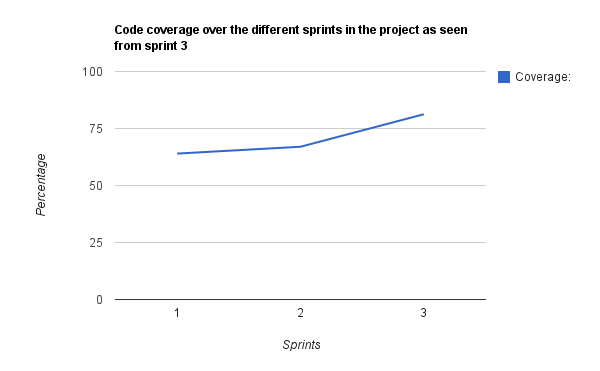
\includegraphics[width=\textwidth]{./sprints/img/sprint3_code_coverage_chart.png}
	\caption{Code coverage progress from previous sprints\label{fig:sp3CoverageChart}}
\end{figure}


%--------------------------
\section{Customer Feedback}
%--------------------------
\label{sec:sp3:feedback}
This section covers the feedback we have got from the customer during the 
spring, with the feedback they gave the team for each of the implemented 
features.

\subsection{Pre-sprint}
The customer was satisfied with the functionality we implemented in sprint 2.
They feel that we are flexible and adapt well to their needs.
Some of the features from sprint 2 were postponed to sprint 3 because we needed additional feedback from the customer.
These include \gls{endianness} and completing the handling of custom \Gls{lua} files.

\subsubsection{New requirements}
We have assigned all the remaining requirements in the product backlog for this sprint.
If we are able to complete all the implementation tasks, the customer will provide us with more requirements for sprint 4.
The customer wants our \gls{utility} to be as automatic as possible, and with as little configuration as possible. 
Additional requirements for sprint 4 will address optimization of the \gls{utility}.

\subsection{During sprint}
In sprint 3 we again demonstrated our \gls{utility} to the customer, and as a result we got some feedback on changes
and improvements we could make. The changes and additions are listed below.

\subsubsection{\Gls{wireshark}, support of search and filter}
To support this the abbreviation field needs to be in place in our code

\subsubsection{\Glspl{struct} within \glspl{struct}}
The customer thought we displayed too much information in the info column in \Gls{wireshark},
 we should only display the name of the outer \gls{struct}.

\subsubsection{Platforms}
We should not generate separate \gls{dissector} files for the different platforms. It is much better if we have one \gls{protocol}
with different functions for the different platforms, as this would not be such a performance hit.

\subsubsection{Flag values}
The customer said that our flag values were inconsistent, some flag values were platform names and some were operating
system names. They suggested using flags such as Solaris-x86, Solaris-SPARC, Win32 and Linux-x86.

\subsubsection{Testing of customer's \gls{header} files}
The customer stressed the importance of our \gls{utility} being able to run on the \gls{header} files they have provided.
Once our \gls{utility} is able to do this they can begin testing the \gls{utility} on their own data.
We can expect to get more feedback on the \gls{utility} when they can fully test it themselves.

\subsection{The backlog and suggestions for sprint 4}
The customer was satisfied with the backlog for sprint 3.
They made several suggestions on features that could improve the \gls{utility}, that we could implement in sprint 4.
These are listed below.

\subsubsection{Unitialized Memory}
It would be nice if our \gls{utility} was able to detect unitialized memory while debugging.
Different compilers use default patterns in \glspl{member} that are unitialized. If our \gls{utility} could detect these patterns,
we could display the data in \Gls{wireshark} with a warning that lets the user know that the data might have been unitialized.

\subsubsection{\Gls{dissector} Ids}
The customer informed us that a \gls{struct} could belong to several \gls{dissector} IDs.
We should implement this by specifying a list of IDs instead of just a single one.

\subsubsection{Include dependency}
The customer describes a scenario where a \gls{struct} is included in another \gls{struct}, which is resident in a different \gls{header} file
that the first \gls{struct} has not included. In this scenario both files are included in a third \gls{header} file.
This creates a dependency which we must take into consideration and implement in the \gls{utility}.

\subsubsection{Specifying file name endings in \gls{batch mode}}
The customer would like to be able to specify the file name endings of the files that are to be created \glspl{dissector} for,
when running the \gls{utility} in \gls{batch mode}. The \gls{utility} only needs to examine \gls{header} files. The \gls{header} files will have one or more known
file extensions, for example, .h and .hpp.

\subsubsection{Overall customer satisfaction}
In general the customer is satisfied with the progress we have made so far. Most of the requirements are
implemented or close to completion. When the \gls{utility} is ready to be tested on their code, we can expect to receive
a lot of feedback on things we need to fix and improve.

%--------------------------
\section{Sprint Evaluation}
%--------------------------
\label{sec:sp3:eval}
After the sprint was finished, the team had an evalution of the sprint. The 
results of this meeting is covered below.

\subsection{Review}
%--------------------------
After some trying, failing and learning we now feel that we understand the \Gls{scrum} process and were able to do it correctly. We have done the planned actions from the prior sprints and have achieved a considerable increase in work efficiency, work completion and now have a well distributed workload.

After not assigning responsibilities at the planning meeting, the team members felt that it was easier to find a task that suited them, which increased the efficiency of task completion. We also listed all the work that needed to be done during the sprint, including meeting, minutes, sprint documentation and so on. This gave us a much better overview of the work.

Looking at the planned actions, we feel that we have managed to do all of them and we are very satisfied with that. The bad experiences mentioned now are only nitpicking compared to the ones in earlier sprints. We see this as a natural evolution, as we learn to do the Scrum steps correctly and efficiently, the team as a whole works better.
But the raised effort from each team member is also indispensable and the improvement we have gained is a result of dedication towards the project.

The burndown chart for the sprint can be seen in \autoref{fig:sp3:burndown}. The estimated and actual hours fit almost flawlessly. This is something we have been good at in all the sprints, but now it is perfected. Even though we estimated too many hours of work for this sprint, all the team members gave their best effort and we almost completed the whole backlog. 
\begin{figure}[!htb]
	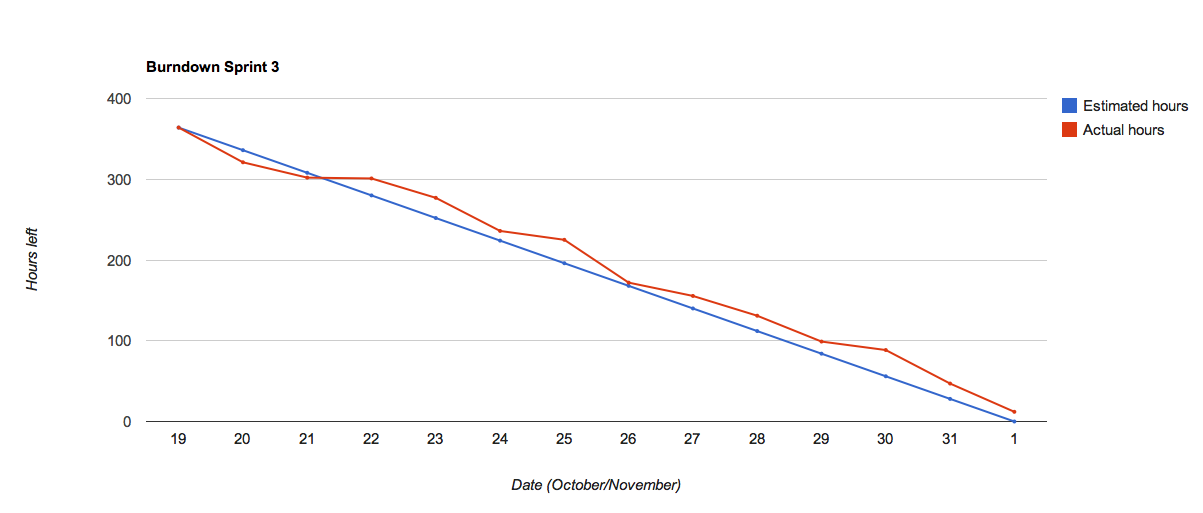
\includegraphics[width=\textwidth]{./sprints/img/burndown_chart_s3}
	\caption{Burndown chart\label{fig:sp3:burndown}}
\end{figure}

\subsection{Positive Experiences}
%--------------------------
\begin{itemize}
	\item Even better planning.
	\item Positive and constructive customer feedback.
	\item The team functions well together.
	\item Planned actions completed.
	\item Easier to pick work items in the backlog after not assigning them at the planning meeting.
	\item Backlog contained all work that had to be done in the sprint. Implementation, documentation, testing and project management.
	\item Team members worked more hours. 
\end{itemize}

\subsection{Negative Experiences}
%--------------------------
\begin{itemize}
	\item The documentation can still be better.
	\item We are not able to finish all tasks in the backlog without working more hours than anticipated.
	\item During the sprint, we had to add work items to the backlog. This is not correct according to \Gls{scrum} procedure, but was necessary because of our lack of knowledge of the domain. This is explained in the barriers section.  
\end{itemize}

\subsection{Planned Actions}
%--------------------------
As mentioned in the review section; we accomplished all the planned actions. The new planned actions are more specific, because this is the last sprint in this project.

\paragraph{Project management}
We have underestimated the hours needed for project management in the prior sprints. We will remember this at the fourth sprint planning meeting and will try to give it a better estimation.
\paragraph{Completion of backlog}
Last sprint means no postponing of work items. We must do a good hour estimation and leave some buffer hours for unforeseen tasks.
\paragraph{Sprint focus}
The next sprint we would like to focus on testing and bug fixing. This is a natural shift, as the project goes into the completion phase. 

\subsection{Barriers}
This sprint the barriers are all concerned with efficiency; bugs, roles and planning.
%--------------------------
\paragraph{Technical problems} 
Unforeseen and undiscovered bugs arise in \Gls{wireshark} while we are developing the \gls{utility}. We report these to the customer, and they patch \Gls{wireshark}'s source code. Our problem is that we have to wait until the customer has made the fix before we can continue.

\paragraph{Product owner}
In \Gls{scrum}, a product owner should be assigned. In our case this is a team member. In a perfect world the product owner would be the customer. The product owner is responsible for prioritizing the product backlog and deciding which work items that should be included in the sprint backlog. We normally use six hours for the sprint planning meeting, and understand that this would be very costly if we were to occupy the customer for this time.

This results in wrong estimates of complexity and we have to add new work items to the backlog during the sprint, as we discover elements that we have overlooked. 

\paragraph{Planning meeting}
It is hard to find a six hour slot where all of the team members can meet. If we do not do the design and proper planning at the planning meeting, we end up with a poor plan. As we get more familiar with \Gls{scrum}, the planning will probably be more efficient and the hours needed will be less. 

